\documentclass[11pt]{article}
\usepackage[utf8]{inputenc}
%Gummi|065|=)
\title{\textbf{Circuitos de rectificaciòn no controlados}}
\author{Cabrera Gutièrrez Raùl\\
		Gutièrrez Olivares Rogelio}
\date{19 de Septiembre del 2019}
\usepackage{graphicx}
\begin{document}
\begin{figure}[htp]
\centering
\includegraphics[scale=1.50]{/home/raulcb/Downloads/th.jpeg}
\caption{logo}
\label{logo}
Universidad Politecnica de la Zona Metropolitana de Gaudalajara.
Sistemas elèctronicos de interfaz.

\end{figure}
\maketitle 

\section{Objetivo}
Analizar el funcionamiento de los rectificadores no controlados.


\section{Materiales}
-Sofware(Orcad)
-Comùtadora
-Guia de trabajo(Hojas con informaciòn necesaria)
\section{Procedimiento}
\maketitle
\textbf{1.2 Rectificadores de media onda con carga inductiv}
Pese a no ser frecuentemente utilizado en la industria, el estudio del rectificador de media onda nos va a permitir poner de manifiesto algunos de los conceptos elementales de la rectificaciòn no controlada. 
por lo que se elavora un diagrama correspondiente a un rectificador de media onda.
\begin{figure}[htp]
\centering
\includegraphics[scale=.20]{/home/raulcb/Documents/media onda.jpeg}
\caption{1.3}
\label{1.3}
\end{figure}


Efectuada la simulaciòn, la forma de la tensiòn rectificada que se aplica a la carga puede observarse la tensiòn de la salida que no sea nula hasta que no lo hace la corriente de carga, como se muestra en la sig figura.
\begin{figure}[htp]
\centering
\includegraphics[scale=0.20]{/home/raulcb/Documents/media rec.jpeg}
\caption{.}
\label{.}
\end{figure}

Esto es debido a que la inductancia de salida se opone a variaciones bruscas de corriente creando una sobretensiòn para mantener al diodo en conducciòn hasta que la corriente se anula.
\\

\maketitle \textbf{1.3 Rectificador monofàsico en puente.}
\\
Estudiamos la principales fromas de onda que caracterizan el funcionamiento y determinan la eleccion de los diodos. Asì mismo, pondremos el contenido armonico que el rectificador produce en la red emperando el factor de potencia.
Otorgando los siguientes valores.
\begin{figure}[htp]
\centering
\includegraphics[scale=0.20]{/home/raulcb/Documents/Mono.jpeg}
\caption{1.4.6}
\label{.}
\end{figure}
\textbf{Rr=10m, Lr=1mH; Lf=1uH; Cf=1mF; Recarga=10}


De esta manera el programa efectuara un analisis sobre la variable que hemos indicadop, esto es la corriente de entrada del rectificador donde se muestra la forma de onda de la tension de salida.
\begin{figure}[htp]
\centering
\includegraphics[scale=.10]{/home/raulcb/Documents/moro recti.jpeg}
\caption{1.5.4}
\label{.}
\end{figure}

\textbf{1.4 Rectificador monofàsico duplicador de tensiòn}
\\
Este tipo de recficador de tension permite obtener en la salida una tension que corresponde aproximadamente al doble. De esta manera es posible obtener tensiones elevadas en la etapa de continuidad sin la necesidad de utilizar un transformador que eleve la tension d entrada del rectificador lo que corresponde al siguiente circuito.
\begin{figure}[htp]
\centering
\includegraphics[scale=0.30]{/home/raulcb/Documents/duplicador.jpeg}
\caption{1.4.7}
\label{.}
\end{figure}
\\
\begin{figure}[htp]
\centering
\includegraphics[scale=0.20]{/home/raulcb/Documents/duplicadormono.jpeg}
\caption{1.4.8}
\label{.}
\end{figure}
\\
Como muestra la imagen las formas de onda de la tensiòn de salida de este rectificador, asì como la que puede medrise en bornes de los condensadores en ellas se puede verificar que el valor medido de la tensiòn rectificada coincide con el doble de la tensiòn.
\\
\\
\\
\\
\\
\\
\\
\\
\\
\\\\
\textbf{1.5 Efecto de los rectificadores monofasicos en lineas trifasicas}
\\

En el siguiente circuito se trabaj el conjunto de tres receptores monofasicos de igual potencia conectados entre cada uno de las fases y el neutro de la instalaciòn como en el siguiente diagrama. 
\begin{figure}[htp]
\centering
\includegraphics[scale=0.10]{/home/raulcb/Documents/Tri.jpeg}
\caption{1.5}
\label{.}
\end{figure}
\\
Las corrientes que circulan por el neutro no es nula pese que los receptores monofasicos esten equilibrados es decir debido a la no linealidad de los receptores, la suma de las tres corrientes de fase no es nula resultando en una corriente de neutro significativamente superior a la corriente de linea.
\begin{figure}[htp]
\centering
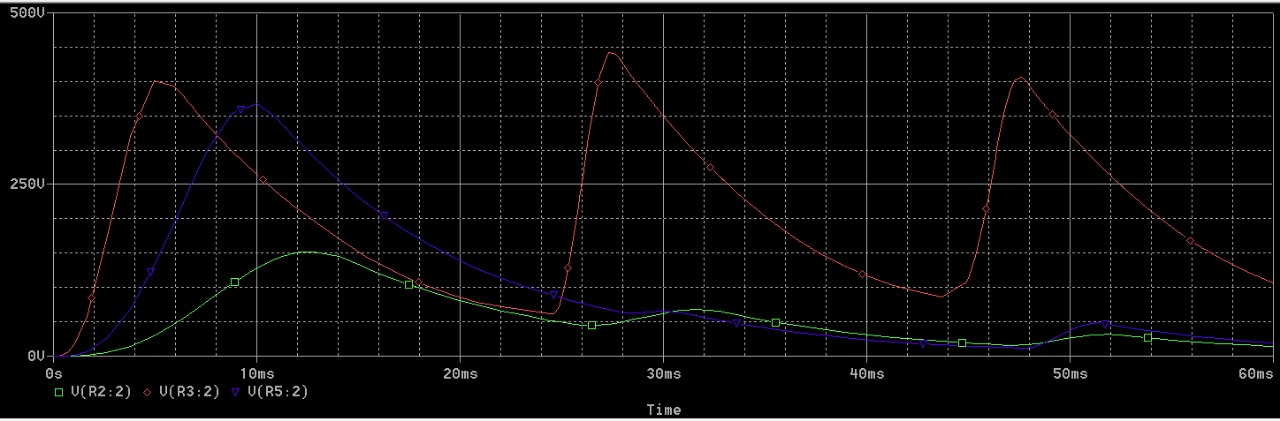
\includegraphics[scale=0.20]{/home/raulcb/Documents/trif.jpeg}
\caption{1.5}
\label{.}
\end{figure}

\textbf{1.6 Rectificadores trifasicos}
\\
Los circuitos trifasicos son utilizados cuando la potencia que consumen de la red es elevada ya que en estos casos la utilizacionde rectificadores monofasicos probocarian desequilibrio importantes en el consumo de las fases.
\begin{figure}[htp]
\centering
\includegraphics[scale=0.20]{/home/raulcb/Documents/trifasico.jpeg}
\caption{1.6}
\label{.}
\end{figure}
\\
Como muestra el esquema elrectificador trifasico no controlado que funciona alimentado por una red de frecuencia 50Hz y 380V eficaz entres fases. 
\begin{figure}[htp]
\centering
\includegraphics[scale=0.20]{/home/raulcb/Documents/trifasico01.jpeg}
\caption{1.6}
\label{.}
\end{figure}
\\
\textbf{1.7 Efecto de las inductancias de red sobre la conmutacion de corriente}
\\
Cuando se añade un inductor de filtro en la etapa de continua, las inductancias de la liena provoca que la conmutacion de corriente entre los diodos no sea instantanea para poner en practica el fenomeno de la conmutacion de corriente entre diodos y analizar sus efectos sobre el funcionamiento del rectificador, como en el siguiente circuito.
\begin{figure}[htp]
\centering
\includegraphics[scale=0.60]{/home/raulcb/Documents/inductancia.jpeg}
\caption{1.7}
\label{.}
\end{figure}
\\\\\\\\\\\\\\\\\\\\\\\\\\\
La inductancia no admite continuidades bruscas en la corriente que circula por ella de manera que mantiene simultaneamnetea los dos diodos en conduccion duarnte un tiempo no despreciable\begin{figure}[htp]
\centering
\includegraphics[scale=0.20]{/home/raulcb/Documents/conmutacion.jpeg}
\caption{1.7}
\label{.}
\end{figure}

\textbf{Conclusiòn}
Los rectificadores son una herramienta escencial para trabajar con circuitos no controlados para calcular de una manera mas sencilla el comportamiento del voltaje y la corriente que pase por el mismo.
 \\
 Como analisamos los distintos tipos de de rectificadores esto aplia el panorama de aplicacion de los mismos dentro de los trabajos y proyectos abriendo una puerta a nuevas idea o propuestas en las cuales trabajar y asi mismo mejorar nuestro desempeño.


\end{document}
